
\section{Shear Wave in a Bar}

This suite of examples focuses on the dynamics of a shear wave propagating
down an 8 km-long bar with a 400 m-wide cross-section. Motion is limited
to shear deformation by fixing the longitudinal degree of freedom.
For each cell type (tri3, quad4, tet4, and hex8) we generate a shear
wave using a kinematic fault rupture with simultaneous slip over the
fault surface, which we place at the center of the bar. The discretization
size is 200 m in all cases. The slip-time histories follow the integral
of Brune's far-field time function with slip initiating at 0.1 s,
a left-lateral final slip of 1.0 m, and a rise time of 2.0 s. The
shear wave speed in the bar is 1.0 km/s, so the shear wave reaches
each end of the bar at 4.1 s. Absorbing boundaries on the ends of
the bar prevent significant reflections. The bar comes to a rest with
a static offset.

\begin{figure}
\begin{centering}
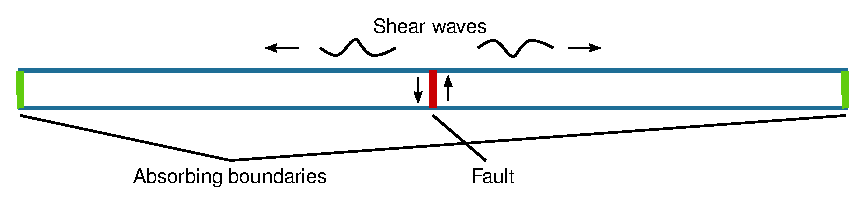
\includegraphics{tutorials/shearwave/figs/bar}
\par\end{centering}

\caption{Domain for shear wave propagation in a 8.0 km bar with 400 m cross-section.
We generate a shear wave via slip on a fault located in the middle
of the bar while limiting deformation to the transverse direction.\label{fig:shearwave:domain}}
\end{figure}


For the bar discretized with quad4 cells we also consider the fault
subjected to frictional sliding controlled by static friction, linear
slip-weakening friction, and rate- and state-friction. We use initial
tractions applied to the fault to drive the dislocation and generate
the shear wave. Because the fault tractions are constant in time,
they continue to drive the motion even after the shear wave reaches
the absorbing boundary, leading to a steady state solution with uniform
shear deformation in the bar and a constant slip rate on the fault. 


\section{\label{sec:tutorial:shearwave:tri3}2D Bar Discretized with Triangles}

PyLith features discussed in this tutorial:
\begin{itemize}
\item Dynamic solution
\item CUBIT format
\item Absorbing dampers boundary conditions
\item Kinematic fault interface conditions
\item Plane strain linearly elastic material
\item VTK output
\item Linear triangular cells
\item SimpleDB spatial database
\item ZeroDispDB spatial database
\end{itemize}
All of the files necessary to run the examples are contained in the
directory \texttt{examples/bar\_shearwave/tri3.}


\subsection{Mesh Generation}

The mesh is a simple rectangle 8 km by 400 m (Figure \vref{fig:shearwave:tet4:mesh}).
This mesh could be generated via a simple script, but it is even easier
to generate this mesh using CUBIT. We provide documented journal files
in \texttt{examples/bar\_shearwave/tri3.} We first create the geometry,
mesh the domain using triangular cells, and then create blocks and
nodesets to associate the cells and vertices with materials and boundary
conditions. See Section \vref{sec:Tutorial-3d-hex8} for more information
on using CUBIT to generate meshes.

\noindent \begin{center}
\begin{figure}
\begin{centering}
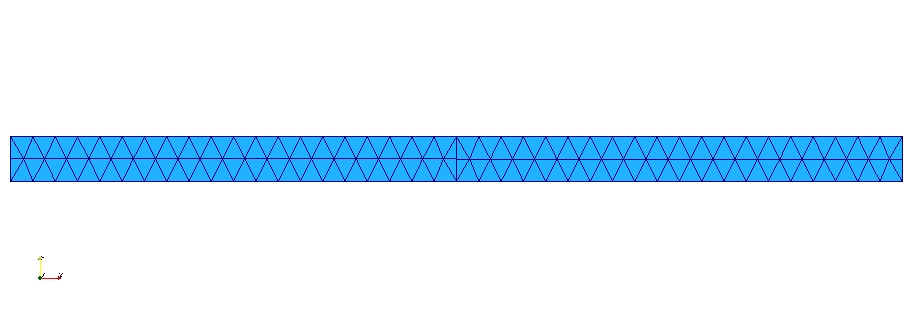
\includegraphics[scale=0.5]{tutorials/shearwave/figs/tri3mesh}
\par\end{centering}

\caption{Mesh composed of triangular cells generated by CUBIT used for the
example problem.\label{fig:shearwave:tri3:mesh}}
\end{figure}

\par\end{center}


\subsection{Simulation Parameters}

All of the parameters are set in the \texttt{pylithapp.cfg} file.
The structure of the file follows the same pattern as in all of the
other examples. We set the parameters for the journal information
followed by the mesh reader, problem, materials, boundary conditions,
fault, and output. We change the time-stepping formulation from the
default value of implicit time stepping to explicit time stepping
with a lumped Jacobian matrix by setting the formulation object via
\begin{lyxcode}
formulation~=~pylith.problems.Explicit
\end{lyxcode}
Using the Explicit object automatically triggers lumping of the Jacobian
cell matrices and assembly into a vector rather than a sparse matrix.
Lumping the Jacobian decouples the equations, so we can use a very
simple direct solver. Use of this simple solver is also triggered
by the selection of any of the Explicit formulation objects. 

For dynamic problems we use the NondimElasticDynamic object to nondimensionalize
the equations. This object provides scales associated with wave propagation
for nondimensionalization, including the minimum wave period, the
shear wave speed, and mass density. In this example we use the default
values of a minimum wave period of 1.0 s, a shear wave speed of 3
km/s, and a mass density of 3000 kg/m$^{3}$. We simulate 12.0 s of
motion with a time step of 1/30 s. This time step must follow the
Courant\textendash{}Friedrichs\textendash{}Lewy condition; that is,
the time step must be smaller than the time it takes the P wave to
propagate across the shortest edge of a cell. 

The boundary conditions include the absorbing dampers at the ends
of the bar and a Dirichlet boundary condition to prevent longitudinal
motion. Because we cannot overlap the Dirichlet BC with the fault,
we use the nodeset associated with all vertices except the fault.
For the output over the entire domain, we request both displacement
and velocity fields:
\begin{lyxcode}
{[}pylithapp.timedependent.output{]}

vertex\_data\_fields~=~{[}displacement,velocity{]}
\end{lyxcode}
To run the problem, simply run PyLith without any command line arguments:
\begin{lyxcode}
pylith
\end{lyxcode}
The VTK files will be written to the \texttt{output} directory. The
output includes the displacement and velocity fields over the entire
domain at every 3rd time step (0.10 s), the slip and change in traction
vectors on the fault surface in along-strike and normal directions
at every 3rd time step (0.10 s), and the strain and stress tensors
for each cell at every 30th time step (1.0 s). If the problem ran
correctly, you should be able to generate a figure such as Figure
\vref{fig:shearwave:tri3:deform}, which was generated using ParaView.

\noindent \begin{center}
\begin{figure}
\begin{centering}
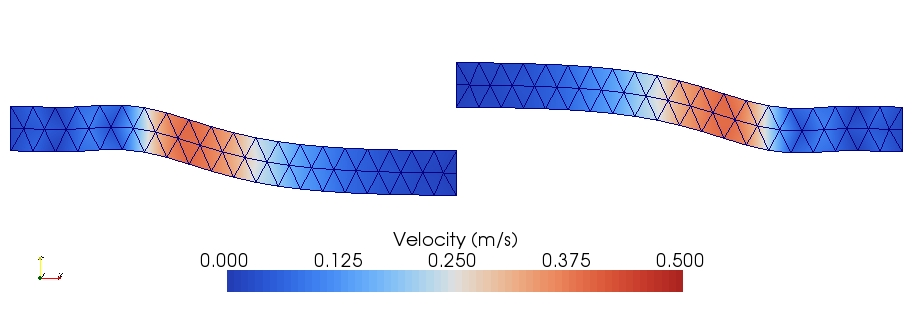
\includegraphics[scale=0.5]{tutorials/shearwave/figs/tri3deform30}
\par\end{centering}

\caption{Displacement field in the bar at 3.0 s. Deformation has been exaggerated
by a factor of 800.\label{fig:shearwave:tri3:deform}}
\end{figure}

\par\end{center}

\section{\label{sec:tutorial:shearwave:tet4}3D Bar Discretized with Tetrahedra}

PyLith features discussed in this tutorial:
\begin{itemize}
\item Dynamic solution
\item LaGriT mesh format
\item Absorbing dampers boundary conditions
\item Kinematic fault interface conditions
\item Elastic isotropic linearly elastic material
\item VTK output
\item Linear tetrahedral cells
\item SimpleDB spatial database
\item ZeroDispDB spatial database
\end{itemize}
All of the files necessary to run the examples are contained in the
directory \texttt{examples/bar\_shearwave/tet4.}


\subsection{Mesh Generation}

The mesh is a simple rectangular prism 8 km by 400 m by 400m (Figure
\vref{fig:shearwave:tet4:mesh}). This mesh could be generated via
a simple script, but it is even easier to generate this mesh using
LaGriT. We provide documented LaGriT files in \texttt{examples/bar\_shearwave/tet4.}
We first create the geometry and regions, mesh the domain using tetrahedral
cells, and then create point sets associated with boundary conditions.

\noindent \begin{center}
\begin{figure}
\begin{centering}
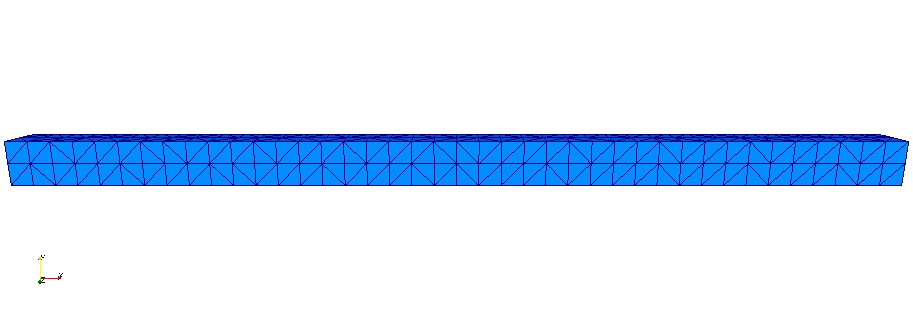
\includegraphics[scale=0.5]{tutorials/shearwave/figs/tet4mesh}
\par\end{centering}

\caption{Mesh composed of tetrahedral cells generated by LaGriT used for the
example problem.\label{fig:shearwave:tet4:mesh}}
\end{figure}

\par\end{center}


\subsection{Simulation Parameters}

The simulation parameters match those in the tri3 example with the
exception of using the LaGriT mesh reader and switching from a two-dimensional
problem to a three-dimensional problem. In addition to fixing the
longitudinal degree of freedom, we also fix the out-of-plane transverse
degree of freedom. Because the fault separates two material regions
in LaGriT, we use two materials in PyLith. All of the parameters are
set in the \texttt{pylithapp.cfg} file. To run the problem, simply
run PyLith without any command line arguments:
\begin{lyxcode}
pylith
\end{lyxcode}
The VTK files will be written to the \texttt{output} directory. The
output includes the displacement and velocity fields over the entire
domain at every 3rd time step (0.10 s), the slip and change in traction
vectors on the fault surface in along-strike and normal directions
at every 3rd time step (0.10 s), and the strain and stress tensors
for each cell at every 30th time step (1.0 s). If the problem ran
correctly, you should be able to generate a figure such as Figure
\vref{fig:shearwave:tet4:deform}, which was generated using ParaView.

\noindent \begin{center}
\begin{figure}
\begin{centering}
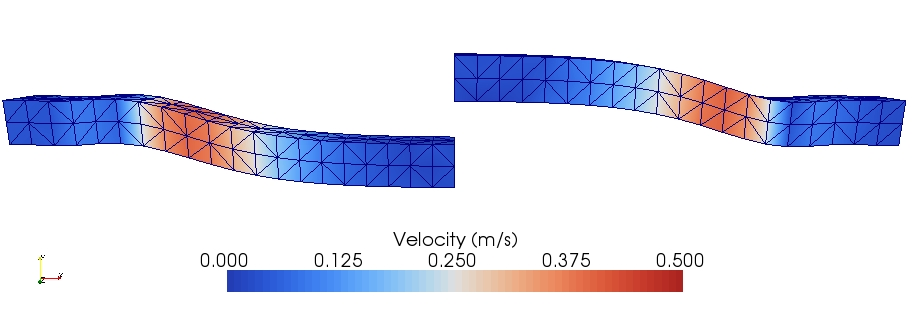
\includegraphics[scale=0.5]{tutorials/shearwave/figs/tet4deform30}
\par\end{centering}

\caption{Displacement field in the bar at 3.0 s. Deformation has been exaggerated
by a factor of 800.\label{fig:shearwave:tet4:deform}}
\end{figure}

\par\end{center}

\section{\label{sec:tutorial:shearwave:hex8}3D Bar Discretized with Hexahedra}

PyLith features discussed in this tutorial:
\begin{itemize}
\item Dynamic solution
\item CUBIT mesh format
\item Absorbing dampers boundary conditions
\item Kinematic fault interface conditions
\item Elastic isotropic linearly elastic material
\item VTK output
\item Linear hexahedral cells
\item SimpleDB spatial database
\item ZeroDispDB spatial database
\end{itemize}
All of the files necessary to run the examples are contained in the
directory \texttt{examples/bar\_shearwave/hex8.}


\subsection{Mesh Generation}

The mesh is a simple rectangular prism 8 km by 400 m by 400 m (Figure
\ref{fig:shearwave:hex8:mesh}). This mesh could be generated via
a simple script, but it is even easier to generate this mesh using
CUBIT. We provide documented CUBIT journal files in \texttt{examples/bar\_shearwave/hex8.}
We first create the geometry, mesh the domain using hexahedral cells,
and then create blocks and nodesets associated with the materials
and boundary conditions.

\noindent \begin{center}
\begin{figure}
\begin{centering}
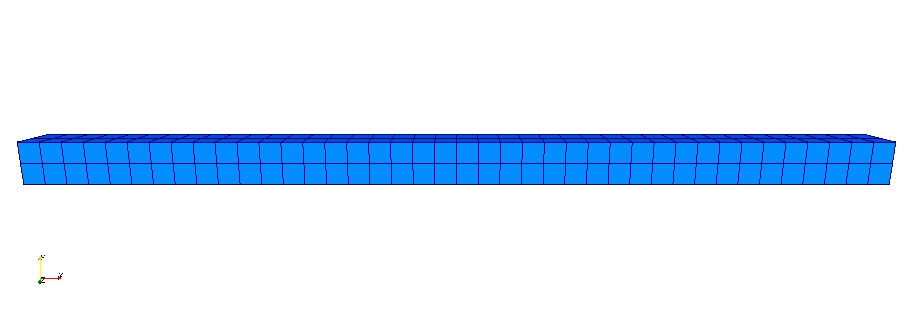
\includegraphics[scale=0.5]{tutorials/shearwave/figs/hex8mesh}
\par\end{centering}

\caption{Mesh composed of hexahedral cells generated by CUBIT used for the
example problem.\label{fig:shearwave:hex8:mesh}}
\end{figure}

\par\end{center}


\subsection{Simulation Parameters}

The simulation parameters match those in the tri3 and tet4 examples.
As in the tet4 example, we fix both the longitudinal degree of freedom
and the out-of-plane transverse degree of freedom. Using eight-point
quadrature permits use of a time step of 1/20 s, which is slightly
larger than the time step of 1/30 s used in the tri3 and tet4 simulations.
All of the parameters are set in the \texttt{pylithapp.cfg} file.
To run the problem, simply run PyLith without any command line arguments:
\begin{lyxcode}
pylith
\end{lyxcode}
The VTK files will be written to the \texttt{output} directory. The
output includes the displacement and velocity fields over the entire
domain at every other time step (0.10 s), the slip and change in traction
vectors on the fault surface in along-strike and normal directions
at every other time step (0.10 s), and the strain and stress tensors
for each cell at every 20th time step (1.0 s). If the problem ran
correctly, you should be able to generate a figure such as Figure
\ref{fig:shearwave:hex8:deform}, which was generated using ParaView.

\noindent \begin{center}
\begin{figure}
\begin{centering}
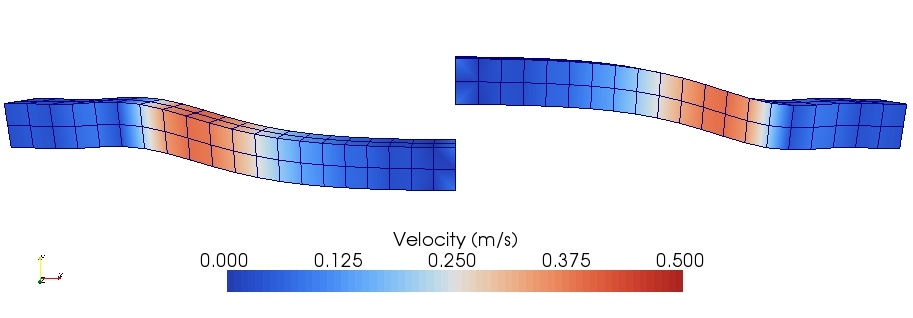
\includegraphics[scale=0.5]{tutorials/shearwave/figs/hex8deform30}
\par\end{centering}

\caption{Displacement field in the bar at 3.0 s. Deformation has been exaggerated
by a factor of 800.\label{fig:shearwave:hex8:deform}}
\end{figure}

\par\end{center}

\section{\label{sec:tutorial:shearwave:quad4}3D Bar Discretized with Quadrilaterals}

PyLith features discussed in this tutorial:
\begin{itemize}
\item Dynamic solution
\item CUBIT mesh format
\item Absorbing dampers boundary conditions
\item Kinematic fault interface conditions
\item Dynamic fault interface conditions
\item Plane strain linearly elastic material
\item VTK output
\item Linear quadrilateral cells
\item SimpleDB spatial database
\item ZeroDispDB spatial database
\item UniformDB spatial database
\end{itemize}
All of the files necessary to run the examples are contained in the
directory \texttt{examples/bar\_shearwave/quad4.}


\subsection{Mesh Generation}

The mesh is a simple rectangular prism 8 km by 400 m by 400 m (Figure
\vref{fig:shearwave:quad4:mesh}). We provide documented CUBIT journal
files in \texttt{examples/bar\_shearwave/quad4.} We first create the
geometry, mesh the domain using quadrilateral cells, and then create
blocks and nodesets associated with the materials and boundary conditions.

\noindent \begin{center}
\begin{figure}
\begin{centering}
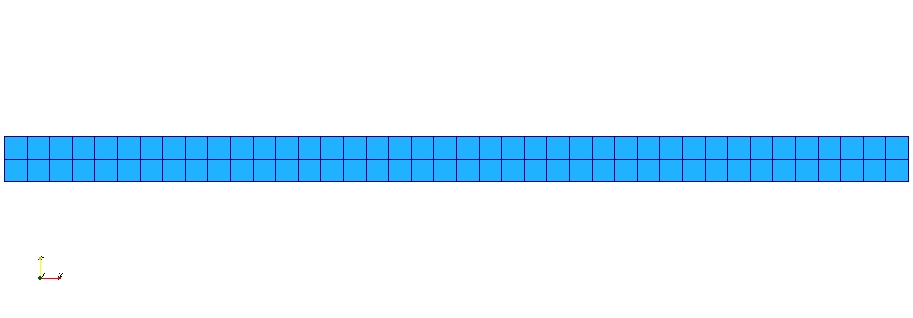
\includegraphics[scale=0.5]{tutorials/shearwave/figs/quad4mesh}
\par\end{centering}

\caption{Mesh composed of hexahedral cells generated by CUBIT used for the
example problem.\label{fig:shearwave:quad4:mesh}}
\end{figure}

\par\end{center}


\subsection{Kinematic Fault (Prescribed Slip)}

The simulation parameters match those in the tri3, tet4, and hex8
examples. Using four-point quadrature permits use of a time step of
1/20 s, which is slightly larger than the time step of 1/30 s used
in the tri3 and tet4 simulations. In contrast to the tri3, tet4, and
hex8 shear wave examples which only contained a single simulation
in a directory, in this example we consider several different simulations.
Consequently, we separate the parameters into multiple \texttt{.cfg}
files. The common parameters are placed in \texttt{pylithapp.cfg}
with the parameters specific to the kinematic fault (prescribed rupture)
example in \texttt{prescribedrup.cfg}. To run the problem, simply
run PyLith via:
\begin{lyxcode}
pylith~prescribedrup.cfg
\end{lyxcode}
The VTK files will be written to the \texttt{output} directory with
the pvrefix \texttt{prescribedrup}. The output includes the displacement
field over the entire domain at every other time step (0.10 s), the
slip and traction vectors on the fault surface in along-strike and
normal directions at every other time step (0.10 s), and the strain
and stress tensors for each cell at every 20th time step (1.0 s).
If the problem ran correctly, you should be able to generate a figure
such as Figure \vref{fig:shearwave:quad4:kinematic}, which was generated
using ParaView.

\noindent \begin{center}
\begin{figure}
\begin{centering}
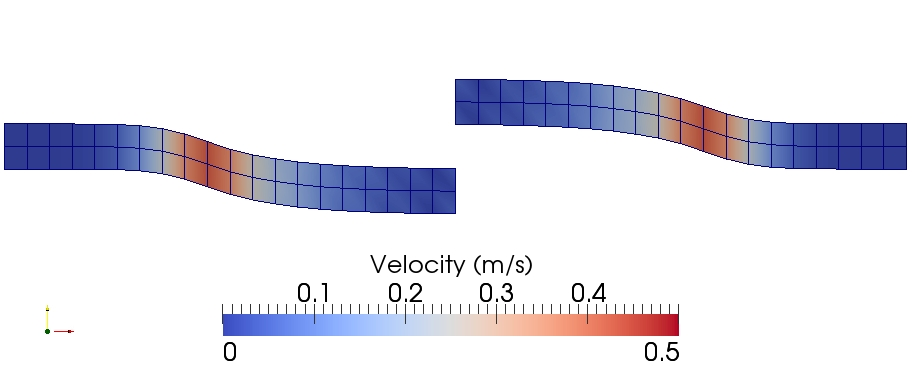
\includegraphics[scale=0.5]{tutorials/shearwave/figs/quad4kinematic30}
\par\end{centering}

\caption{Displacement field in the bar at 3.0 s. Deformation has been exaggerated
by a factor of 800.\label{fig:shearwave:quad4:kinematic}}
\end{figure}

\par\end{center}


\subsection{Dynamic Fault (Spontaneous Rupture)}

In this set of examples we replace the kinematic fault interface with
the dynamic fault interface, resulting in fault slip controlled by
a fault-constitutive model. See Section \vref{sec:fault:constitutive:models}
for detailed information about the fault constitutive models available
in PyLith. Because this is a dynamic simulation we want the generated
shear wave to continue to be absorbed at the ends of the bar, so we
drive the fault by imposing initial tractions directly on the fault
surface rather than through deformation within the bar. We impose
initial tractions (75 MPa of right-lateral shear and 120 MPa of compression)
plus a temporal variation (smoothly increasing from 0 to 25 MPa of
right-lateral shear) similar to what would be used in a 2-D or 3-D
version. While the magnitude of these stresses is reasonable for tectonic
problems, they give rise to very large slip rates in this 1-D bar.
The temporal variation, as specified via the \texttt{traction\_change.timedb}
file, has the functional form:
\begin{equation}
f(t)=\begin{cases}
\exp\left(\frac{\left(t-t_{n}\right)^{2}}{t\left(t-2t_{n}\right)}\right), & 0<t\le t_{n}\\
1, & t>t_{n}
\end{cases}
\end{equation}
where $t_{n}$ = 1.0 s. We request that the fault output include the
initial traction value and the slip, slip rate, and traction fields:
\begin{lyxcode}
{[}pylithapp.timedependent.interfaces.fault.output{]}

vertex\_info\_fields={[}traction\_initial\_value{]}

vertex\_data\_fields~=~{[}slip,slip\_rate,traction{]}
\end{lyxcode}
The steady-state solution for this problem is constant velocity and
slip rate with uniform strain within the bar. A Python script, \texttt{analytical\_soln.py},
is included for computing values related to the steady-state solution.


\subsubsection{Dynamic Fault with Static Friction}

The parameters specific to this example involve the static friction
fault constitutive model. We set the fault constitutive model via
\begin{lyxcode}
{[}pylithapp.timedependent.interfaces.fault{]}

friction~=~pylith.friction.StaticFriction
\end{lyxcode}
and use a UniformDB to set the static friction parameters. We use
a coefficient of friction of 0.6 and no cohesion (0 MPa). The parameters
specific to this example are in \texttt{spontaneousrup\_staticfriction.cfg},
so we run the problem via:
\begin{lyxcode}
pylith~spontaneousrup.cfg~spontaneousrup\_staticfriction.cfg
\end{lyxcode}
The VTK files will be written to the \texttt{output} directory with
the pvrefix \texttt{staticfriction}. The output includes the displacement
and velocity fields over the entire domain at every other time step
(0.10 s), the slip, slip rate, and traction vectors on the fault surface
in along-strike and normal directions at every other time step (0.10
s), and the strain and stress tensors for each cell at every 20th
time step (1.0 s). If the problem ran correctly, you should be able
to generate a figure such as Figure \vref{fig:shearwave:quad4:staticfriction},
which was generated using ParaView. The steady-state solution is a
constant slip rate of 22.4 m/s, a shear traction of 72.0 MPa on the
fault surface, a uniform shear strain of 5.6e-3 in the bar with uniform,
and constant velocities in the y-direction of +11.2 m/s and -11.2
m/s on the -x and +x sides of the fault, respectively.

\noindent \begin{center}
\begin{figure}
\begin{centering}
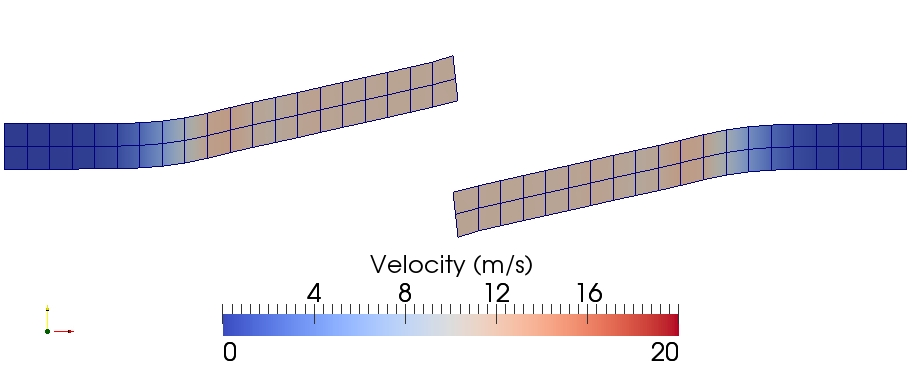
\includegraphics[scale=0.5]{tutorials/shearwave/figs/quad4staticfriction30}
\par\end{centering}

\caption{Velocity field in the bar at 3.0 s for the static friction fault constitutive
model. Deformation has been exaggerated by a factor of 20.\label{fig:shearwave:quad4:staticfriction}}
\end{figure}

\par\end{center}


\subsubsection{Dynamic Fault with Slip-Weakening Friction}

The parameters specific to this example are related to the use of
the slip-weakening friction fault constitutive model (see Section
\vref{sec:fault:constitutive:models}). We set the fault constitutive
model via
\begin{lyxcode}
{[}pylithapp.timedependent.interfaces.fault{]}

friction~=~pylith.friction.SlipWeakening
\end{lyxcode}
and use a UniformDB to set the slip-weakening friction parameters.
We use a static coefficient of friction of 0.6, a dynamic coefficient
of friction of 0.5, a slip-weakening parameter of 0.2 m, and no cohesion
(0 MPa). The fault constitutive model is associated with the fault,
so we can append the fault constitutive model parameters to the vertex
information fields:
\begin{lyxcode}
{[}pylithapp.timedependent.interfaces.fault.output{]}

vertex\_info\_fields~=~{[}strike\_dir,normal\_dir,initial\_traction,static\_coefficient,~\\
dynamic\_coefficient,slip\_weakening\_parameter,cohesion{]}
\end{lyxcode}
The parameters specific to this example are in \texttt{spontaneousrup\_slipweakening.cfg},
so we run the problem via:
\begin{lyxcode}
pylith~spontaneousrup.cfg~spontaneousrup\_slipweakening.cfg
\end{lyxcode}
The VTK files will be written to the \texttt{output} directory with
the pvrefix \texttt{slipweakening}. If the problem ran correctly, you
should be able to generate a figure such as Figure \vref{fig:shearwave:quad4:slipweakening},
which was generated using ParaView. The steady-state solution is a
constant slip rate of 32.0 m/s and shear traction of 60.0 MPa on the
fault surface, a uniform shear strain of 8.0e-3 in the bar with uniform,
constant velocities in the y-direction of +16.0 m/s and -46.0 m/s
on the -x and +x sides of the fault, respectively.

\noindent \begin{center}
\begin{figure}
\begin{centering}
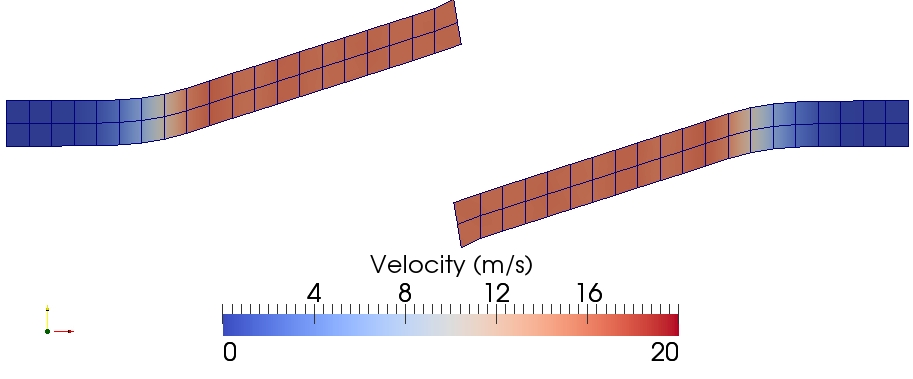
\includegraphics[scale=0.5]{tutorials/shearwave/figs/quad4slipweakening30}
\par\end{centering}

\caption{Velocity field in the bar at 3.0 s for the slip-weakening friction
fault constitutive model. Deformation has been exaggerated by a factor
of 20.\label{fig:shearwave:quad4:slipweakening}}
\end{figure}

\par\end{center}


\subsubsection{Dynamic Fault with Rate-State Friction}

The parameters specific to this example are related to the use of
the rate- and state-friction fault constitutive model (see Section
\vref{sec:fault:constitutive:models}). The evolution of the state
variable uses the ageing law. We set the fault constitutive model
and add the state variable to the output via
\begin{lyxcode}
{[}pylithapp.timedependent.interfaces.fault{]}

friction~=~pylith.friction.RateStateAgeing~\\


{[}pylithapp.timedependent.interfaces.fault.output{]}~\\
vertex\_data\_fields~=~{[}slip,~slip\_rate,~traction,~state\_variable{]}~
\end{lyxcode}
and use a UniformDB to set the rate-state friction parameters. We
use a vreference coefficient of friction of 0.6, vreference slip rate
of 1.0e-6 m/s, characteristic slip distance of 0.02 m, coefficients
a and b of 0.008 and 0.012, and no cohesion (0 MPa). We set the initial
value of the state variable so that the fault is in equilibrium for
the initial tractions. The parameters specific to this example are
in \texttt{spontaneousrup\_ratestateageing.cfg}, so we run the problem
via:
\begin{lyxcode}
pylith~spontaneousrup.cfg~spontaneousrup\_ratestateageing.cfg
\end{lyxcode}
The VTK files will be written to the \texttt{output} directory with
the pvrefix \texttt{ratestateageing}. If the problem ran correctly,
you should be able to generate a figure such as Figure \vref{fig:shearwave:quad4:ratestateageing},
which was generated using ParaView. The steady-state solution is a
constant slip rate of 30.0 m/s and shear traction of 63.7 MPa on the
fault surface, a uniform shear strain of 7.25e-3 in the bar with uniform,
constant velocities in the y-direction of +15.0 m/s and -15.0 m/s
on the -x and +x sides of the fault, respectively.

\noindent \begin{center}
\begin{figure}
\begin{centering}
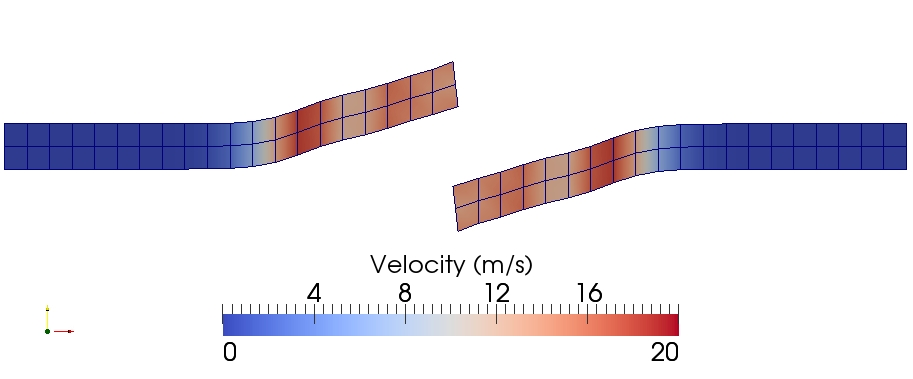
\includegraphics[scale=0.5]{tutorials/shearwave/figs/quad4ratestateageing30}
\par\end{centering}

\caption{Velocity field in the bar at 3.0 s for the rate- and state-friction
fault constitutive model. Deformation has been exaggerated by a factor
of 20.\label{fig:shearwave:quad4:ratestateageing}}
\end{figure}

\par\end{center}

